\chapter{Interconnection Networks}
\label{ch:networks}

Whatever the memory organisation, processors (or processors and memory) have to be \emph{connected}. In a
shared-memory machine the interconnect joins processors to memory modules; in a distributed-memory machine it joins
processors to each other. As machines grow, the interconnect is often what limits performance, so it deserves careful study.

\section{What an interconnect is made of}
\slides{20--22}

An interconnect has a few kinds of building blocks.

\begin{definition}{network interface, link, switch}
A \textbf{network interface} connects a processor (or memory) to the network. In a cluster this is the network card, attached to the
processor over PCI or PCI-e, the expansion bus of the computer. A \textbf{link} is a set of wires or an optical fibre carrying data between two points.
A \textbf{switch} has several input \emph{ports} and output \emph{ports} and forwards data arriving on an input to the appropriate
output. The number of ports is the switch's \emph{degree}.
\end{definition}

The slide describes the \term{communication network} as switching elements to which the processors are attached through ports; the switching elements are linked
in some \emph{pattern}, and that pattern is the \term{topology}. (In shared-memory machines the memory modules are
attached to the network too.)

It helps to think of the whole interconnect as a \emph{graph}: the nodes are processors, memories and switches, and the edges are links. A \emph{hop} is one link traversed,
and the \emph{distance} between two nodes is the number of links on the shortest path between them.

\section{Static and dynamic networks}
\slides{23--24}

\begin{definition}{static (direct) network}
Fixed, point-to-point links connect the processing nodes directly to each other. Each node can be thought of as a processor
together with its own small switch (router). Examples: ring, mesh, torus, hypercube.
\end{definition}

\begin{definition}{dynamic (indirect) network}
Processors (and memories) are attached to \emph{switches}, and the switches make connections on demand. Paths are
formed dynamically by setting the switches. Examples: crossbar, Omega network, fat tree.
\end{definition}

\begin{center}
\begin{tikzpicture}
  % static
  \node[font=\small\bfseries] at (1.2,2.6) {static (direct)};
  \foreach \i/\x/\y in {1/0/0, 2/2.4/0, 3/2.4/1.8, 4/0/1.8} {
     \node[pe] (a\i) at (\x,\y) {$P_\i$};
  }
  \draw[lnk] (a1) -- (a2) -- (a3) -- (a4) -- (a1);
  % dynamic
  \node[font=\small\bfseries] at (8,2.6) {dynamic (indirect)};
  \foreach \i/\x in {1/6.2,2/7.4,3/8.6,4/9.8} {
     \node[pe] (b\i) at (\x,0) {$P_\i$};
     \node[swt] (s\i) at (\x,1.0) {};
     \draw[lnk] (b\i) -- (s\i);
  }
  \node[swt,fill=gray!35] (t1) at (6.8,2.0) {}; \node[swt,fill=gray!35] (t2) at (9.2,2.0) {};
  \draw[lnk] (s1) -- (t1) -- (s2); \draw[lnk] (s3) -- (t2) -- (s4); \draw[lnk] (t1) -- (t2);
\end{tikzpicture}
\end{center}

\section{How a message travels: a cost model and routing}
\slides{23}

This section goes slightly beyond the slides, but it explains \emph{why} the quantities the slides define (diameter, bisection width) matter.

\subsection{A simple cost model}

Suppose a message of $m$ words crosses $l$ links. Three constants describe the machine:
$t_s$, the \emph{startup time} (software overhead and setting up the transfer, paid once per message, independent of $m$);
$t_h$, the time for the message's header to pass through one switch (per-hop delay);
and $t_w$, the time to transfer one word over a link ($1/t_w$ is the bandwidth).

\begin{itemize}
  \item \textbf{Store-and-forward}: each switch receives the whole message and only then forwards it:
        $T = t_s + l\,(t_h + m\,t_w)$.
  \item \textbf{Cut-through (wormhole) routing}: the message is cut into small pieces that are pipelined along the path, like cars on a road; the head
        moves on while the tail is still leaving the source: $T = t_s + l\,t_h + m\,t_w$.
\end{itemize}

\begin{workedex}{store-and-forward versus cut-through}
$m=1000$ words, $t_w=1$, $t_h=10$, $t_s=100$ (arbitrary time units), $l=5$ links.
\[
  T_{\text{SF}} = 100 + 5(10+1000) = 5150, \qquad T_{\text{CT}} = 100 + 5\cdot 10 + 1000 = 1150 .
\]
With cut-through, the long message pays the transfer time $m\,t_w$ only \emph{once}, and distance adds only a little.
\end{workedex}

Two lessons: for \emph{short} messages the startup and hop count dominate, so a small \emph{diameter} helps; for \emph{long}
messages the bandwidth term dominates. And whenever many messages must cross the same part of the network, the total traffic
divided by the available bandwidth across that cut is a lower bound on the time. That is what \emph{bisection bandwidth}
(below) measures.

\subsection{Routing}

\term{Routing} decides which path a message takes from source to destination (the slide: ``how the route taken by the message
from source to destination is decided'').
\begin{itemize}
  \item \textbf{Deterministic} routing always uses the same path for a given source and destination. A common form is
        \emph{dimension-ordered routing}: in a 2-D mesh, move along the $x$ direction until the column matches, then along $y$.
        It is simple and avoids \emph{deadlock} (a cycle of messages each waiting for a resource held by the next) on meshes.
  \item \textbf{Adaptive} routing chooses among several paths according to current congestion; it spreads load but is harder to build.
\end{itemize}

\section{Static topologies}
\slides{24, 28--31}

\subsection{Completely connected, star, linear array and ring}

\begin{center}
\begin{tikzpicture}[scale=0.9]
  % complete graph
  \foreach \i in {0,...,5} \node[dn] (k\i) at ({60*\i}:1) {};
  \begin{pgfonlayer}{background}
  \foreach \i in {0,...,5} \foreach \j in {0,...,5} { \ifnum\i<\j \draw (k\i) -- (k\j); \fi }
  \end{pgfonlayer}
  \node[font=\scriptsize,align=center] at (0,-1.7) {completely\\connected};
  % star
  \begin{scope}[shift={(3.6,0)}]
    \node[dn,fill=orange!30] (h) at (0,0) {};
    \foreach \i in {0,...,5} \node[dn] (s\i) at ({60*\i+30}:1) {};
    \begin{pgfonlayer}{background}\foreach \i in {0,...,5} \draw (h) -- (s\i);\end{pgfonlayer}
    \node[font=\scriptsize] at (0,-1.7) {star};
  \end{scope}
  % linear array
  \begin{scope}[shift={(5.9,0)}]
    \foreach \i in {0,...,4} \node[dn] (l\i) at (0.65*\i,0.4) {};
    \draw (l0) -- (l1) -- (l2) -- (l3) -- (l4);
    \node[font=\scriptsize] at (1.3,-0.35) {linear array};
    \foreach \i in {0,...,4} \node[dn] (r\i) at (0.65*\i,-1.4) {};
    \draw (r0) -- (r1) -- (r2) -- (r3) -- (r4);
    \draw[dashed] (r0) to[bend right=45] (r4);
    \node[font=\scriptsize,align=center] at (1.3,-2.5) {linear array with\\wraparound = ring};
  \end{scope}
\end{tikzpicture}
\end{center}

\begin{itemize}
  \item \textbf{Completely connected}: every node has a direct link to every other, so any message goes in one hop and
        no pair blocks another. It is the static counterpart of the crossbar, with the same flaw: the number of links is
        $p(p-1)/2$, which is hopeless for large $p$.
  \item \textbf{Star}: all nodes connect to a central node that acts as a switch. Diameter 2, but the central node is a bottleneck (similar to a bus).
  \item \textbf{Linear array}: nodes in a line, each linked to its two neighbours. A \textbf{ring} (also a ``1-D torus'') adds a
        \emph{wraparound} link between the two ends. The wraparound halves the diameter and doubles the number of routes.
\end{itemize}

\subsection{Meshes and tori}

\begin{center}
\begin{tikzpicture}
  \foreach \i in {0,...,3} \foreach \j in {0,...,3} { \node[dn] (m\i\j) at (1.0*\i,1.0*\j) {}; }
  \foreach \i in {0,...,3} \foreach \j in {0,...,2} { \draw (m\i\j) -- (m\i\the\numexpr\j+1\relax); }
  \foreach \i in {0,...,2} \foreach \j in {0,...,3} { \draw (m\i\j) -- (m\the\numexpr\i+1\relax\j); }
  \foreach \j in {0,...,3} \draw[dashed,gray] (m3\j) to[bend left=20] (m0\j);
  \foreach \i in {0,...,3} \draw[dashed,gray] (m\i0) to[bend right=20] (m\i3);
  \node[font=\small,align=center] at (1.5,-0.9) {$4\times4$ mesh (solid) and torus\\(solid $+$ dashed wraparound links)};
\end{tikzpicture}
\end{center}

A \term{2-D mesh} arranges $p$ nodes in a $\sqrt p\times\sqrt p$ grid; node $(i,j)$ is linked to $(i\pm1,j)$ and $(i,j\pm1)$.
It is easy to lay out on a chip or board (it is planar) and it maps naturally onto computations on grids (images, stencils). A \term{torus} adds wraparound
links in each dimension. Extending to three dimensions gives a 3-D mesh/torus, where interior nodes have $6$ neighbours; 3-D simulations map naturally onto it.

\begin{definition}{$k$-ary $d$-cube / $k$-$d$ mesh}
A network with $d$ dimensions and $k$ nodes along each dimension, so $p=k^{d}$ nodes. A linear array is $d=1$, a 2-D mesh $d=2$. With wraparound links it is a
$k$-ary $d$-cube (a torus).
\end{definition}

\subsection{Hypercubes}

A hypercube is the case $k=2$: two nodes per dimension and $d=\log_2 p$ dimensions (the slide writes ``$2$-$\log p$ mesh'').

\begin{center}
\begin{tikzpicture}[x=1.4cm,y=1.2cm]
  \node[dn,minimum size=8mm] (n000) at (0,0)     {\tiny 000};
  \node[dn,minimum size=8mm] (n001) at (2,0)     {\tiny 001};
  \node[dn,minimum size=8mm] (n011) at (2,2)     {\tiny 011};
  \node[dn,minimum size=8mm] (n010) at (0,2)     {\tiny 010};
  \node[dn,minimum size=8mm] (n100) at (1,0.9)   {\tiny 100};
  \node[dn,minimum size=8mm] (n101) at (3,0.9)   {\tiny 101};
  \node[dn,minimum size=8mm] (n111) at (3,2.9)   {\tiny 111};
  \node[dn,minimum size=8mm] (n110) at (1,2.9)   {\tiny 110};
  \begin{pgfonlayer}{background}
  \draw (n000)--(n001)--(n011)--(n010)--(n000);
  \draw (n100)--(n101)--(n111)--(n110)--(n100);
  \draw (n000)--(n100) (n001)--(n101) (n011)--(n111) (n010)--(n110);
  \end{pgfonlayer}
\end{tikzpicture}
\end{center}

\textbf{Construction and numbering.} A $d$-dimensional hypercube is built from \emph{two} $(d-1)$-dimensional hypercubes by joining each node of one to the
corresponding node of the other. If you prefix the labels of one copy with $0$ and the other with $1$, you get the numbering in the figure.

\begin{keyidea}
\textbf{Two nodes are neighbours exactly when their labels differ in one bit}, and the distance between any two nodes equals the number of
bits in which their labels differ (the \emph{Hamming distance}). Example: $0110$ and $0101$ differ in two bits, so they are two links apart.
\end{keyidea}

This gives the routing rule (\emph{e-cube routing}): to go from $a$ to $b$, look at $a\oplus b$ (bitwise exclusive-or) and flip the differing bits one at a time.
It also gives the diameter: labels have $\log_2 p$ bits, so at most $\log_2 p$ flips are needed. The cost is that each node needs $\log_2 p$ links,
which grows with machine size, and many parallel algorithms (reductions, sorting, FFT) are designed to exploit this structure.

\subsection{Trees and fat trees}

\begin{center}
\begin{tikzpicture}[level distance=0.9cm,
   level 1/.style={sibling distance=3.2cm},level 2/.style={sibling distance=1.5cm},
   every node/.style={}]
  % static tree
  \node[dn] at (1.7,2.0) (r) {};
  \foreach \x/\p in {0.35/a,3.05/b} { \node[dn] (\p) at (\x+0.0,1.1) {}; \draw (r) -- (\p); }
  \foreach \x/\p/\q in {-0.4/c/a,1.1/d/a,2.3/e/b,3.8/f/b} { \node[dn] (\p) at (\x,0.2) {}; \draw (\q) -- (\p); }
  \node[font=\scriptsize] at (1.7,-0.45) {static tree (every node is a processor)};
  % dynamic tree
  \begin{scope}[shift={(6.6,0)}]
  \node[swt] at (1.7,2.0) (R) {};
  \foreach \x/\p in {0.35/A,3.05/B} { \node[swt] (\p) at (\x,1.1) {}; \draw (R) -- (\p); }
  \foreach \x/\p/\q in {-0.4/C/A,1.1/D/A,2.3/E/B,3.8/F/B} { \node[pe,minimum width=5mm,minimum height=5mm,font=\scriptsize] (\p) at (\x,0.2) {P}; \draw (\q) -- (\p); }
  \node[font=\scriptsize] at (1.7,-0.45) {dynamic tree (processors at the leaves)};
  \end{scope}
\end{tikzpicture}
\end{center}

A tree has exactly one path between any two nodes. In a \emph{static} tree every node is a processor; in a \emph{dynamic} tree
the inner nodes are switches and the processors are the leaves (the slide notes that ``our campus network'' is a tree).
Routing is easy: send the message \emph{up} to the lowest common ancestor of source and destination, then \emph{down}.

The weakness is the top: all messages between the left and right halves must pass through the root, which becomes the bottleneck.

\begin{definition}{fat tree}
A tree in which \emph{links get thicker towards the root}: the number of links between a node and its parent equals the number of links from that node down to its
children (the slide's ``fundamental property''). In a binary tree with one link per leaf, a switch one level above the leaves has $2$ links up, the next
level $4$, and so on.
\end{definition}

\begin{center}
\begin{tikzpicture}[sw/.style={draw,fill=gray!25,minimum width=7mm,minimum height=4mm}]
  \foreach \i in {0,...,7} \node[pe,minimum width=5mm,minimum height=5mm,font=\scriptsize] (l\i) at (1.2*\i,0) {P};
  \foreach \i in {0,...,3} \node[sw] (a\i) at (2.4*\i+0.6,1.3) {};
  \foreach \i in {0,1} \node[sw] (b\i) at (4.8*\i+1.8,2.6) {};
  \node[sw] (c) at (4.2,3.9) {};
  \foreach \i in {0,...,3} { \draw[line width=0.6pt] (l\the\numexpr2*\i\relax) -- (a\i); \draw[line width=0.6pt] (l\the\numexpr2*\i+1\relax) -- (a\i); }
  \foreach \i/\k in {0/0,1/0,2/1,3/1} { \draw[line width=1.6pt] (a\i) -- (b\k); }
  \foreach \i in {0,1} { \draw[line width=3.2pt] (b\i) -- (c); }
\end{tikzpicture}
\end{center}

Because the capacity towards the root keeps pace with the number of processors below, \emph{any} pair of processors can communicate at full
speed without contention: a fat tree is a \emph{non-blocking} network. Its bisection width grows in proportion to $p$ (cutting at the root severs $p/2$ links' worth of
capacity), so the bisection bandwidth \emph{per node} stays constant. The slide calls these \term{constant bisection bandwidth} (CBB) networks.
A two-level fat tree has diameter $4$ (leaf, switch, root, switch, leaf: four links). In practice, thick links are built from many ordinary
links and identical small switches; most commodity clusters use a fat-tree-like network.

\section{Dynamic networks}
\slides{25--27}

\subsection{Bus}

A \term{bus} is a single set of wires shared by all attached devices. Only one transfer can take place at a time. Cost grows
linearly with the number of nodes and any two nodes are one ``hop'' apart, but the \emph{total} bandwidth is fixed, so each node's share falls as $1/p$. A bus
(or a ring, as the slide adds) is used only in small shared-memory systems. Local caches help by keeping most accesses off the bus. A bus is also what makes snooping
possible (Chapter~\ref{ch:coherence}): everything is naturally broadcast.

\subsection{Crossbar}

\begin{center}
\begin{tikzpicture}[x=1.2cm,y=1.0cm]
  \foreach \i in {0,...,3} { \node[mm,minimum width=8mm] (M\i) at (\i,3.9) {$M_\i$}; \node[pe,minimum width=8mm] (P\i) at (-1.1,3-\i) {$P_\i$}; }
  \foreach \i in {0,...,3} { \draw[gray] (\i,3.6) -- (\i,-0.3); \draw[gray] (-0.7,3-\i) -- (3.3,3-\i); }
  \foreach \i in {0,...,3} \foreach \j in {0,...,3} { \draw[fill=white] (\i-0.07,3-\j-0.07) rectangle (\i+0.07,3-\j+0.07); }
  \draw[fill=red!60] (2-0.1,3-0-0.1) rectangle (2+0.1,3-0+0.1);
  \draw[fill=red!60] (0-0.1,3-1-0.1) rectangle (0+0.1,3-1+0.1);
  \draw[fill=red!60] (3-0.1,3-2-0.1) rectangle (3+0.1,3-2+0.1);
  \draw[fill=red!60] (1-0.1,3-3-0.1) rectangle (1+0.1,3-3+0.1);
  \node[font=\scriptsize,align=left,anchor=west] at (3.6,1.5) {red = closed switches:\\$P_0{-}M_2$, $P_1{-}M_0$,\\$P_2{-}M_3$, $P_3{-}M_1$\\(all four at once)};
\end{tikzpicture}
\end{center}

A \term{crossbar} connects $p$ processors to $b$ memory banks with a $p\times b$ grid of switching elements. Each crossing can
either connect or isolate its row wire and its column wire. A processor reaches any memory by closing the switch at the crossing of its row and the
memory's column.

\begin{itemize}
  \item \textbf{Non-blocking}: connecting one processor to one memory never prevents any other processor from connecting to any other \emph{free} memory. Any permutation can be realised at once, as in the figure.
  \item \textbf{Cost}: $\Theta(pb)$ switches. Usually $b\ge p$ so that every processor can find a free bank, so the cost is at least $\Omega(p^{2})$.
        This is why crossbars suit only small or medium machines (and why they are used inside switch chips): performance scales,
        \emph{cost} does not.
\end{itemize}

\subsection{Multistage networks and the Omega network}

A \term{multistage network} sits between the bus (cheap, low performance) and the crossbar (high performance, expensive): several stages of small
switches, traded for fewer switches than a crossbar and more bandwidth than a bus. The slide's example is the \term{Omega network}.

\textbf{Structure.} With $p$ inputs (processors) and $p$ outputs (memory banks), the Omega network has $\log_2 p$ \emph{stages}, each made of $p/2$
two-input, two-output switches. Each switch is in one of two settings: \emph{pass-through} (inputs go straight to the outputs) or \emph{cross-over}
(the two are swapped). The wiring between stages (and into the first stage) is the \term{perfect shuffle}: input $i$ is connected to output
\[
  j = \begin{cases} 2i & 0\le i\le p/2-1,\\ 2i+1-p & p/2\le i\le p-1,\end{cases}
\]
which is the same as rotating the binary representation of $i$ one position to the left. For $p=8$: $001\to010$, $010\to100$,
$101\to011$, and $000$, $111$ map to themselves.

\textbf{Why $\log_2 p$ stages?} Each stage can decide one bit of the destination address; with $p=2^k$ destinations you need $k$ decisions.

\textbf{Routing.} To send from source $s$ to destination $t$, both written in binary with the most significant bit first: at stage $k$ ($k=1,2,\dots$), compare the
$k$-th bit of $s$ with the $k$-th bit of $t$. If they are \emph{equal}, the switch is set to pass-through; if they \emph{differ}, to cross-over. After $\log_2 p$
stages the message arrives at $t$.

\begin{workedex}{routing in an $8\times 8$ Omega network}
Route $010\to111$: compare bit by bit: $0$ vs $1$ differ $\Rightarrow$ cross; $1$ vs $1$ same $\Rightarrow$ pass; $0$ vs $1$ differ $\Rightarrow$ cross.
Route $110\to100$: $1$ vs $1$ same $\Rightarrow$ pass; $1$ vs $0$ differ $\Rightarrow$ cross; $0$ vs $0$ same $\Rightarrow$ pass.
\end{workedex}

\begin{center}
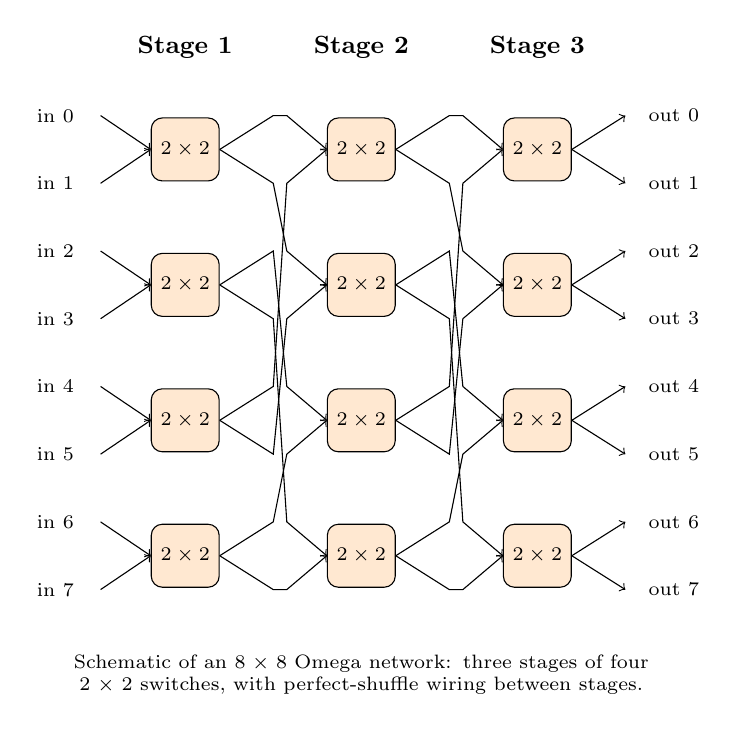
\begin{tikzpicture}[scale=0.86, every node/.style={font=\scriptsize}]
  % Illustrative 8x8 Omega network: three stages, four 2x2 switches per stage.
  \foreach \i in {0,...,7} {
    \node[left] at (0,7-\i) {in \i};
    \node[right] at (8.2,7-\i) {out \i};
  }
  \foreach \s/\x in {1/1.5,2/4.1,3/6.7} {
    \node[font=\small\bfseries] at (\x,8.0) {Stage \s};
    \foreach \j in {0,...,3} {
      \node[draw,rounded corners,fill=orange!18,minimum width=7mm,minimum height=8mm] (sw\s\j) at (\x,6.5-2*\j) {$2\times2$};
    }
  }
  % Inputs to stage 1 (paired adjacent lanes).
  \foreach \i in {0,...,7} {
    \pgfmathtruncatemacro{\j}{int(floor(\i/2))}
    \draw[->] (0.25,7-\i) -- (sw1\j.west);
  }
  % Perfect-shuffle wiring between stages: output lane i goes to input lane (2i mod 7), with 7 fixed.
  \foreach \i in {0,...,7} {
    \pgfmathtruncatemacro{\src}{int(floor(\i/2))}
    \pgfmathtruncatemacro{\k}{ifthenelse(\i==7,7,mod(2*\i,7))}
    \pgfmathtruncatemacro{\j}{int(floor(\k/2))}
    \draw[->] (sw1\src.east) -- (2.8,7-\i) -- (3.0,7-\k) -- (sw2\j.west);
  }
  \foreach \i in {0,...,7} {
    \pgfmathtruncatemacro{\src}{int(floor(\i/2))}
    \pgfmathtruncatemacro{\k}{ifthenelse(\i==7,7,mod(2*\i,7))}
    \pgfmathtruncatemacro{\j}{int(floor(\k/2))}
    \draw[->] (sw2\src.east) -- (5.4,7-\i) -- (5.6,7-\k) -- (sw3\j.west);
  }
  \foreach \i in {0,...,7} {
    \pgfmathtruncatemacro{\j}{int(floor(\i/2))}
    \draw[->] (sw3\j.east) -- (8.0,7-\i);
  }
  \node[align=center,text width=8cm] at (4.1,-1.25) {Schematic of an $8\times8$ Omega network: three stages of four $2\times2$ switches, with perfect-shuffle wiring between stages.};
\end{tikzpicture}

\end{center}

\textbf{Cost.} $\log_2 p$ stages of $p/2$ switches give $\tfrac p2\log_2 p=\Theta(p\log p)$ switches, which lies between the bus ($\Theta(p)$) and the
crossbar ($\Theta(p^{2})$). For $p=1024$: a crossbar has $1024^2=1\,048\,576$ crosspoints; an Omega network has
$512\times 10=5120$ two-by-two switches (a $2\times2$ switch is equivalent to $4$ crosspoints, so about $20\,000$). The number of stages, and hence the latency, grows only as $\log p$.

\textbf{Blocking.} Unlike the crossbar, an Omega network is a \emph{blocking} network: there is exactly \emph{one} path between each input and output, and two messages with
different sources \emph{and} different destinations can still need the same switch output.
The figure shows $010\to100$ (solid blue) and $110\to111$ (dashed red) at the same time. Both arrive at the same first-stage switch and both need its
same output, so one must wait. In the crossbar, the slide's ``non-blocking'' contrast, these two requests would both be served immediately.

\begin{workedex}{how restrictive is blocking?}
An $8\times8$ Omega network has $\tfrac p2\log_2 p=12$ switches, each with $2$ settings, so only $2^{12}=4096$ different switch settings, and each setting
realises a different permutation. But there are $8!=40\,320$ permutations of $8$ inputs onto $8$ outputs. The Omega network can realise only
about $10\%$ of them. For $p=16$ the figures are $2^{32}\approx4.3\times10^{9}$ settings against $16!\approx2.1\times10^{13}$ permutations: about $0.02\%$. (I checked the $p=8$ count by
brute force.) This is the price paid for cutting the switch count.
\end{workedex}

\section{Evaluating networks}
\slides{32--34}

How do we compare topologies? The slides use these criteria.

\begin{definition}{diameter}
The \emph{maximum} distance between any two processing nodes, where distance is the length of the shortest path in links. It bounds the worst-case number
of hops.
\end{definition}

\begin{definition}{connectivity (arc connectivity)}
The \emph{minimum number of links that must be removed} to split the network into two disconnected parts. It measures the number of alternative paths
and the fault tolerance: high connectivity is better.
\end{definition}

\begin{definition}{bisection width}
The \emph{minimum number of links that must be removed} to split the network into two \emph{equal halves}. It measures the
capacity between the two halves in the worst case.
\end{definition}

\begin{definition}{channel width, channel rate, channel bandwidth, bisection bandwidth}
\textbf{Channel width}: the number of bits that a link carries simultaneously, i.e.\ the number of physical wires in it.
\textbf{Channel rate}: the peak rate at which a single wire delivers bits.
\textbf{Channel bandwidth} $=$ channel width $\times$ channel rate.
\textbf{Bisection bandwidth} $=$ bisection width $\times$ channel bandwidth: the maximum volume of communication between the two halves of the network.
\end{definition}

Two further quantities appear in comparisons: the \textbf{degree} (links per node: it determines the hardware each node needs), and the
\textbf{cost}, measured here as the \emph{number of links}.

\subsection{Deriving the values}

\begin{itemize}
  \item \textbf{Diameter.} Completely connected: $1$. Star: $2$ (leaf, hub, leaf). Ring: the farthest node is half-way round, $\lfloor p/2\rfloor$.
        2-D mesh: corner to opposite corner is $(\sqrt p-1)+(\sqrt p-1)=2(\sqrt p-1)$. 2-D torus: wraparound means at most half-way in each
        dimension, $2\lfloor\sqrt p/2\rfloor$. Hypercube: labels have $\log_2 p$ bits, so at most $\log_2 p$ flips. Complete binary tree with $p$ nodes:
        height $\log_2\frac{p+1}{2}$, and the worst pair is two leaves in different subtrees of the root, $2\log_2\frac{p+1}{2}$.
  \item \textbf{Arc connectivity.} Linear array, tree, star: $1$ (one link failing disconnects a node). Ring: $2$. 2-D mesh without wraparound: $2$ (a corner node has only two links).
        Torus: $4$. $d$-dimensional hypercube: $d$ (every node has $d$ links and removing all of them isolates it).
  \item \textbf{Bisection width.} Ring: $2$ (cut the ring in two places). 2-D mesh: $\sqrt p$ (cut the $\sqrt p$ horizontal links crossing the middle column boundary). Torus: $2\sqrt p$ (the
        wraparound links double it). Hypercube: split by one bit; every node on one side has exactly one neighbour on the other, so $p/2$ links cross.
        Completely connected: each of the $p/2$ nodes in one half has a link to each of the $p/2$ in the other, $p^2/4$ links. Tree: $1$ (cut near the root).
  \item \textbf{Cost (links).} Linear array $p-1$; ring $p$; star $p-1$; tree $p-1$; completely connected $p(p-1)/2$; 2-D mesh $2p-2\sqrt p$; 2-D torus $2p$;
        hypercube $(p\log_2 p)/2$ (each of $p$ nodes has $\log_2 p$ links and every link is counted twice); $k$-ary $d$-cube $dp$.
\end{itemize}

\begin{pitfall}
\textbf{About the star's bisection width.} The slides and the textbook table list $1$ for the star, meaning the single link whose removal disconnects the network. If you insisted on splitting
the nodes into two exactly equal halves you would have to cut about $p/2$ links (every leaf on the side without the hub). For exams, use the course value $1$,
but know that it is a convention.
\end{pitfall}

\subsection{Summary table}
\label{sec:summarytable}

\begin{center}
\small
\renewcommand{\arraystretch}{1.3}
\begin{tabular}{@{}lcccc@{}}
\toprule
\textbf{Network} & \textbf{Diameter} & \textbf{Bisection width} & \textbf{Arc connectivity} & \textbf{Cost (links)}\\
\midrule
Completely connected & $1$ & $p^{2}/4$ & $p-1$ & $p(p-1)/2$\\
Star & $2$ & $1$ & $1$ & $p-1$\\
Ring & $\lfloor p/2\rfloor$ & $2$ & $2$ & $p$\\
Linear array & $p-1$ & $1$ & $1$ & $p-1$\\
Complete binary tree & $2\log_2\frac{p+1}{2}$ & $1$ & $1$ & $p-1$\\
2-D mesh (no wraparound) & $2(\sqrt p-1)$ & $\sqrt p$ & $2$ & $2(p-\sqrt p)$\\
2-D torus (wraparound) & $2\lfloor\sqrt p/2\rfloor$ & $2\sqrt p$ & $4$ & $2p$\\
Hypercube & $\log_2 p$ & $p/2$ & $\log_2 p$ & $(p\log_2 p)/2$\\
Wraparound $k$-ary $d$-cube & $d\lfloor k/2\rfloor$ & $2k^{d-1}$ & $2d$ & $dp$\\
\bottomrule
\end{tabular}
\end{center}

\begin{workedex}{sixty-four nodes}
\begin{center}
\small
\begin{tabular}{@{}lccccc@{}}
\toprule
 & Diameter & Bisection width & Links & Degree\\
\midrule
Ring & $32$ & $2$ & $64$ & $2$\\
$8\times8$ mesh & $14$ & $8$ & $112$ & up to $4$\\
$8\times8$ torus & $8$ & $16$ & $128$ & $4$\\
6-D hypercube & $6$ & $32$ & $192$ & $6$\\
Completely connected & $1$ & $1024$ & $2016$ & $63$\\
\bottomrule
\end{tabular}
\end{center}
The torus is a good compromise: twice the links of the ring give a $4\times$ shorter diameter and an $8\times$ larger bisection. The hypercube is
better still but needs more links per node and more total links; the completely connected network is best on every performance measure and
impractical in cost.
\end{workedex}

\begin{workedex}{bisection bandwidth in numbers}
Take the $8\times8$ torus. Suppose each link has channel width $16$ wires and each wire delivers $1$~Gbit/s. Then channel bandwidth $=16\times1=16$~Gbit/s and,
with bisection width $16$, the bisection bandwidth is $16\times16=256$~Gbit/s $=32$~GB/s.
If every one of the $32$ nodes in one half sends $1$~GB to a node in the other half, $32$~GB must cross the cut, which takes at least $32/32=1$~second whatever the algorithm. This is the
sense in which bisection bandwidth bounds the speed of communication-heavy programs.
\end{workedex}

\subsection{The blanks on the slides}

The slides leave the values for you to fill in; for reference (with $P$ nodes):
diameter -- fully connected $1$, star $2$, ring $P/2$, hypercube $\log P$;
connectivity -- linear array $1$, ring $2$, 2-D mesh $2$, 2-D mesh with wraparound $4$, $d$-dimensional hypercube $d$;
bisection width -- ring $2$, $P$-node 2-D mesh $\sqrt P$, tree $1$, star $1$, completely connected $P^2/4$, hypercube $P/2$.

\subsection{Where each network is used}

\begin{itemize}
  \item \textbf{Bus}: small shared-memory systems and inside chips (with caches to reduce traffic).
  \item \textbf{Crossbar}: small shared-memory machines and small-to-medium distributed machines; also inside the switches of larger networks.
  \item \textbf{Multistage (Omega)}: medium-sized machines needing more bandwidth than a bus at lower cost than a crossbar.
  \item \textbf{Mesh/torus}: used in several large supercomputers (for example the IBM Blue Gene series used a 3-D torus; Fujitsu's Tofu interconnect is a multi-dimensional mesh/torus), and natural for grid computations.
  \item \textbf{Fat tree}: the dominant choice in commodity clusters, because it is non-blocking and can be built from standard switches.
  \item \textbf{Hypercube}: historically important (many classic parallel algorithms assume it) but rarely built today because the degree grows with $\log p$.
\end{itemize}

\begin{keyidea}
There is no best topology. Diameter measures latency, bisection width and bandwidth measure how much traffic the network can carry, connectivity measures resilience, and links per node
measure cost. Every design trades these off.
\end{keyidea}

\section*{Exercises}
\addcontentsline{toc}{section}{Exercises}
\begin{enumerate}[label=\textbf{\thechapter.\arabic*},leftmargin=*]
  \item For $p=16$ nodes, compute the diameter, bisection width and number of links of (a) a $4\times4$ mesh and (b) a $4\times4$ torus.
  \item In a $4$-dimensional hypercube, how many hops separate nodes $1011$ and $0110$? Give a path that flips the differing bits from the lowest to the highest.
  \item In a $16\times16$ Omega network, how many stages and how many switches are there? Give the switch settings (pass or cross, by stage) for the route $0101\to1100$.
  \item A binary fat tree has $16$ processors at the leaves. How many levels of switches does it have, and what is its diameter in links?
  \item A $16\times16$ torus ($256$ nodes) has channel width $32$ wires and $2$~Gbit/s per wire. Compute the channel bandwidth and the bisection bandwidth in Gbit/s and GB/s.
  \item Explain why a bus does not ``scale'' even though its cost is only $O(p)$.
  \item Compare a 3-D torus of $4096=16^3$ nodes with a $12$-dimensional hypercube of the same size in diameter, bisection width, number of links and degree.
  \item Using the cost model, how long does a message of $m=10^{4}$ words take over $l=8$ links with store-and-forward and with cut-through ($t_s=100$, $t_h=10$, $t_w=1$)?
\end{enumerate}